\section{Case Studies}
In this section, we use four case studies deployed on HydraMini to show the capabilities of our research platform.

\subsection{Autonomous Driving using End-to-End model}
This case shows how you use our platform for AD using end-to-end model. Several recent research replaces the classic chain of perception, planning, and control with a neural network that directly maps sensor input to control output\cite{bojarski2016end, chi2017deep, eraqi2017end}, a methodology known as end-to-end driving. New approaches based on reinforcement learning are being actively developed\cite{kendall2019learning}. An end-to-end AI model is easy to use since it outputs control commands directly. The model contains mainly CNN and Dense layers\cite{keras}, it maps camera input to control output. The structure of the model is shown in Fig.~\ref{ms}.

\begin{figure}[b]
\centerline{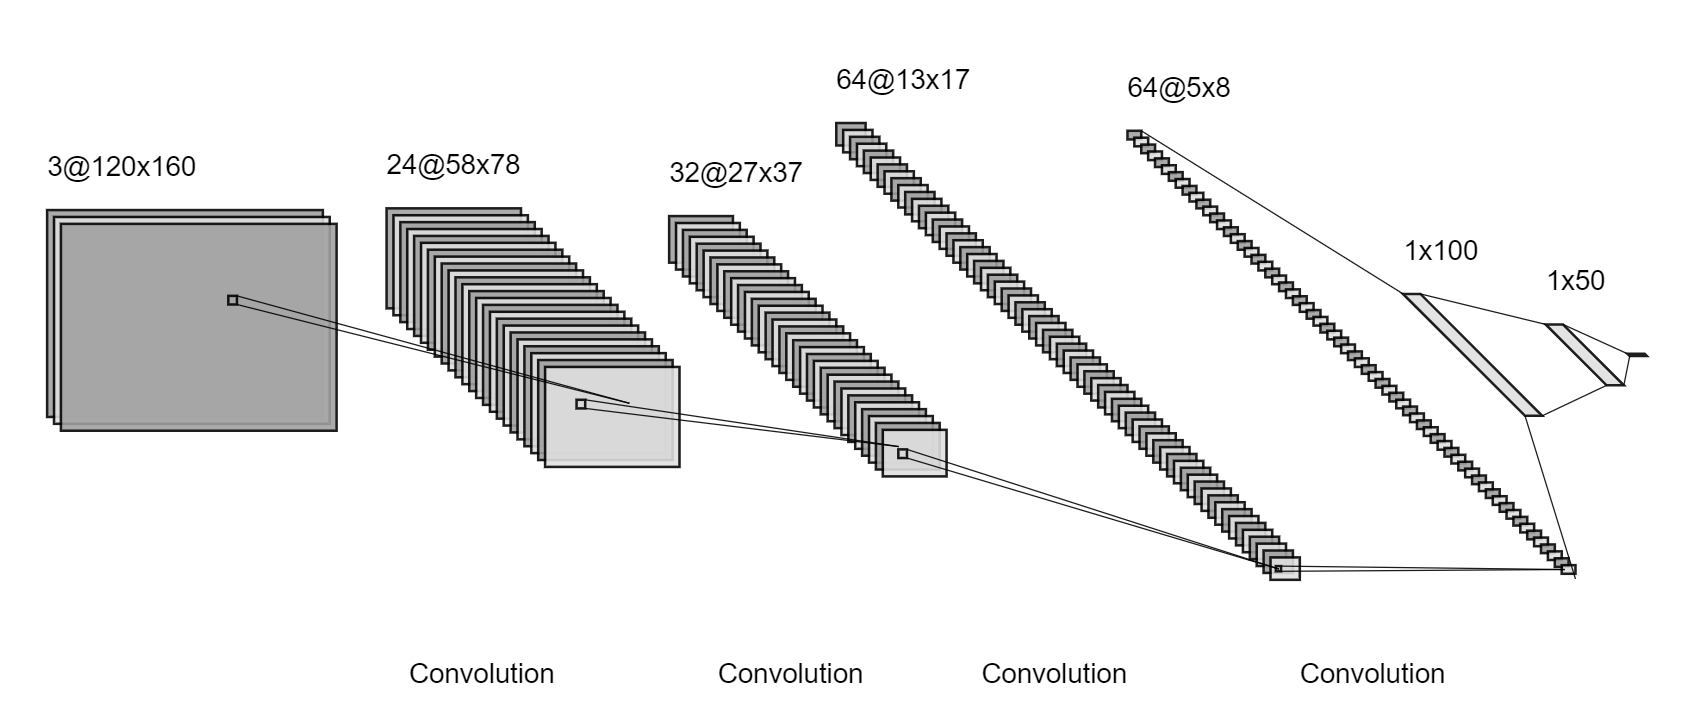
\includegraphics[width=0.5\textwidth]{ns.png}}
\caption{Model Structure.}
\label{ms}
\end{figure}

\begin{figure*}[t]
    \centering
    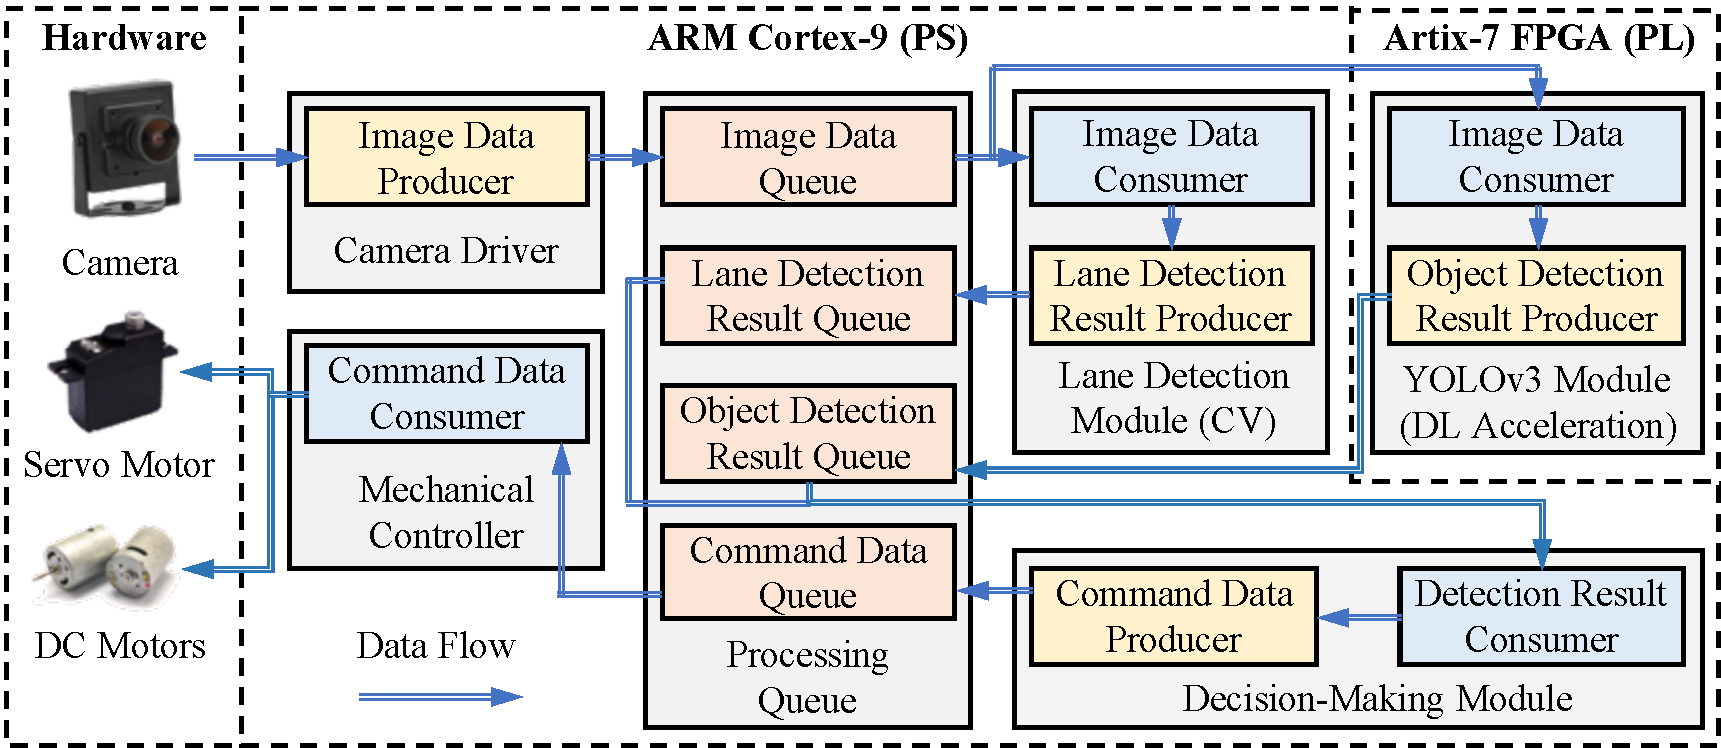
\includegraphics[width=5in]{traditional_autonomous_driving}
    \caption{Autonomous Driving using Traditional Methods.}
    \label{fig:traditional_autonomous_driving}
\end{figure*}

CNN layers extract features from the images taken by the car's front camera. Several fully connected layers follow the CNN layers, they finally extract the command information needed for auto-driving. The activation function we use is Relu. The last layer is a Softmax layer\cite{keras} for classification or a Dense layer for regression. Although the current model is not the perfect one, it's convenient to make changes and do optimizations to the model. Fig.~\ref{fig:end_to_end_autonomous_driving} shows the whole process.

First, you controls the car using your keyboard or whatever you like and save data from the car's sensors as training data. Or you just get the data from Internet or somewhere else. Second, after pre-process, you put the images you get as input to the AI model and the labels such as keyboard signals as the output. Train the model using TensorFlow until you get a satisfactory model. Third, you will use DNNDK\cite{dnndk} provided by Xilinx to do the compression and compilation and then copy the generated files to the car. Finally, the car is able to move by itself. It will be controlled by AI models. 

\begin{figure}[b]
    \centering
    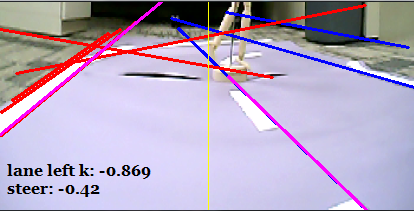
\includegraphics[width=3.5in]{lane_detect}
    \caption{Lane Detection.}
    \label{fig:lane_detection}
\end{figure}

\subsection{Autonomous Driving using traditional methods}
In the first case of AD we use an end-to-end model and in this one we will show you another way of doing AD. This time we will use computer vision methods to detect the road line and use classic YOLOv3 model to find objects.  

To detect road lane, we first use $5 \times 5$ Gaussian filter to remove the noise of the image. Then Canny edge detection\cite{canny1986computational} is applied to detect the edges of the image. Hough transform\cite{burns1986extracting} is employed to detect the lines of the image. Based on the orientation and relative position of detected lines, side line and stop line of the road are identified. To improve the robustness and accuracy of the algorithm, more techniques will be added to the algorithm, such as K-Means clustering\cite{selim1984k} for Hough lines, Kalman/Gabor filtering for sampled data, alternative IPM (inverse perspective mapping) lane detection method\cite{wang2014approach}.

The car will run following the lane of the road, Fig.~\ref{fig:lane_detection} shows the final lanes extracted from all detected lines. The yellow line marks the middle of the picture, the other lines are all lines we find in the photos. Among all the lanes we detected, we will choose one line for both left side and right side and they are painted purple. The red ones and blue ones are the rest. With these information, the car adjusts its direction and speed to the road. For example, in the picture the left lane chosen as the road line has a slope of $-0.869$ which is smaller than the slope datum, then the controller calculated a steer value $-0.42$ and that means to turn left.

\begin{figure}[b]
\centerline{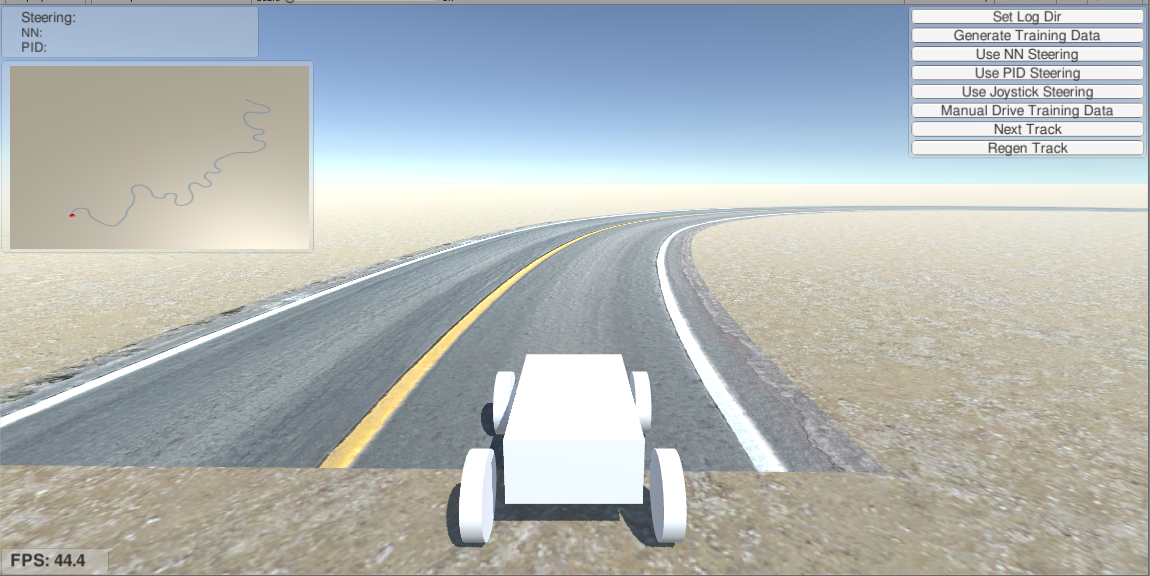
\includegraphics[width=0.5\textwidth]{simulator.png}}
\caption{Simulator Interface.}
\label{si}
\end{figure}

YOLOv3 is used to find objects like people or cars to help the car make decisions like braking to avoid a obstacle. The inference process will be accelerated by DNNDK to meet more stringent real-time requirement, also you could replace full YOLOv3 model with tiny YOLOv3 model to achieve faster inference speed.

Fig.~\ref{fig:traditional_autonomous_driving} shows the control process of this case, the taken images will be processed by both computer vision threads and YOLOv3 threads, this time they won't produce commands directly, instead the information they get will be used to make decisions. Finally, the commands will be generated by the decision maker.

\subsection{Simulator}
The simulator is a tool which helps users test their designs more efficiently. You see the interface of the simulator in Fig.~\ref{fig:lane_detection}. The simulator is based on sdsandbox\cite{sdsandbox} which is a simulator project for Donkey Car\cite{donkeycar}. As you see in the picture, the users use this simulator to collect training data and test their models. 

When testing, you should build a server, the server will receive sensor data from the client of the simulator and generate control messages according to these data. We have already built one example, the server will get images taken by simulator and handles them using the AI model trained before, then the model output control commands and these commands will be sent to the simulator.
It's also convenient for users to modify the source code of the simulator to define their own data format or control methods. However, users should be familiar with C\# and Unity3d if they would like to do so, and we provide coding tutorial manual to help.

\subsection{Lidar in ROS}
Due to the high impact of ROS, we make our platform able to support ROS projects. The version we use is ROS Melodic\cite{rosmelodic} which is mainly used in Ubuntu18.04. 

This time we show how to read LiDAR data and control the car using ROS. With Lidar data, the car is able to handle obstacle avoidance tasks and SLAM tasks whose basical technology is Lidar data processing.
The Lidar we use is LeiShen LS01D\cite{leishen}, LeiShen has already provided one ROS node for users to gain and publish Lidar data. We read the  laser point cloud data by subscribing the published topic. Also, it will be more visualized to use RViz\cite{rviz}, Fig.~\ref{ld} is one example.

\begin{figure}[b]
\centerline{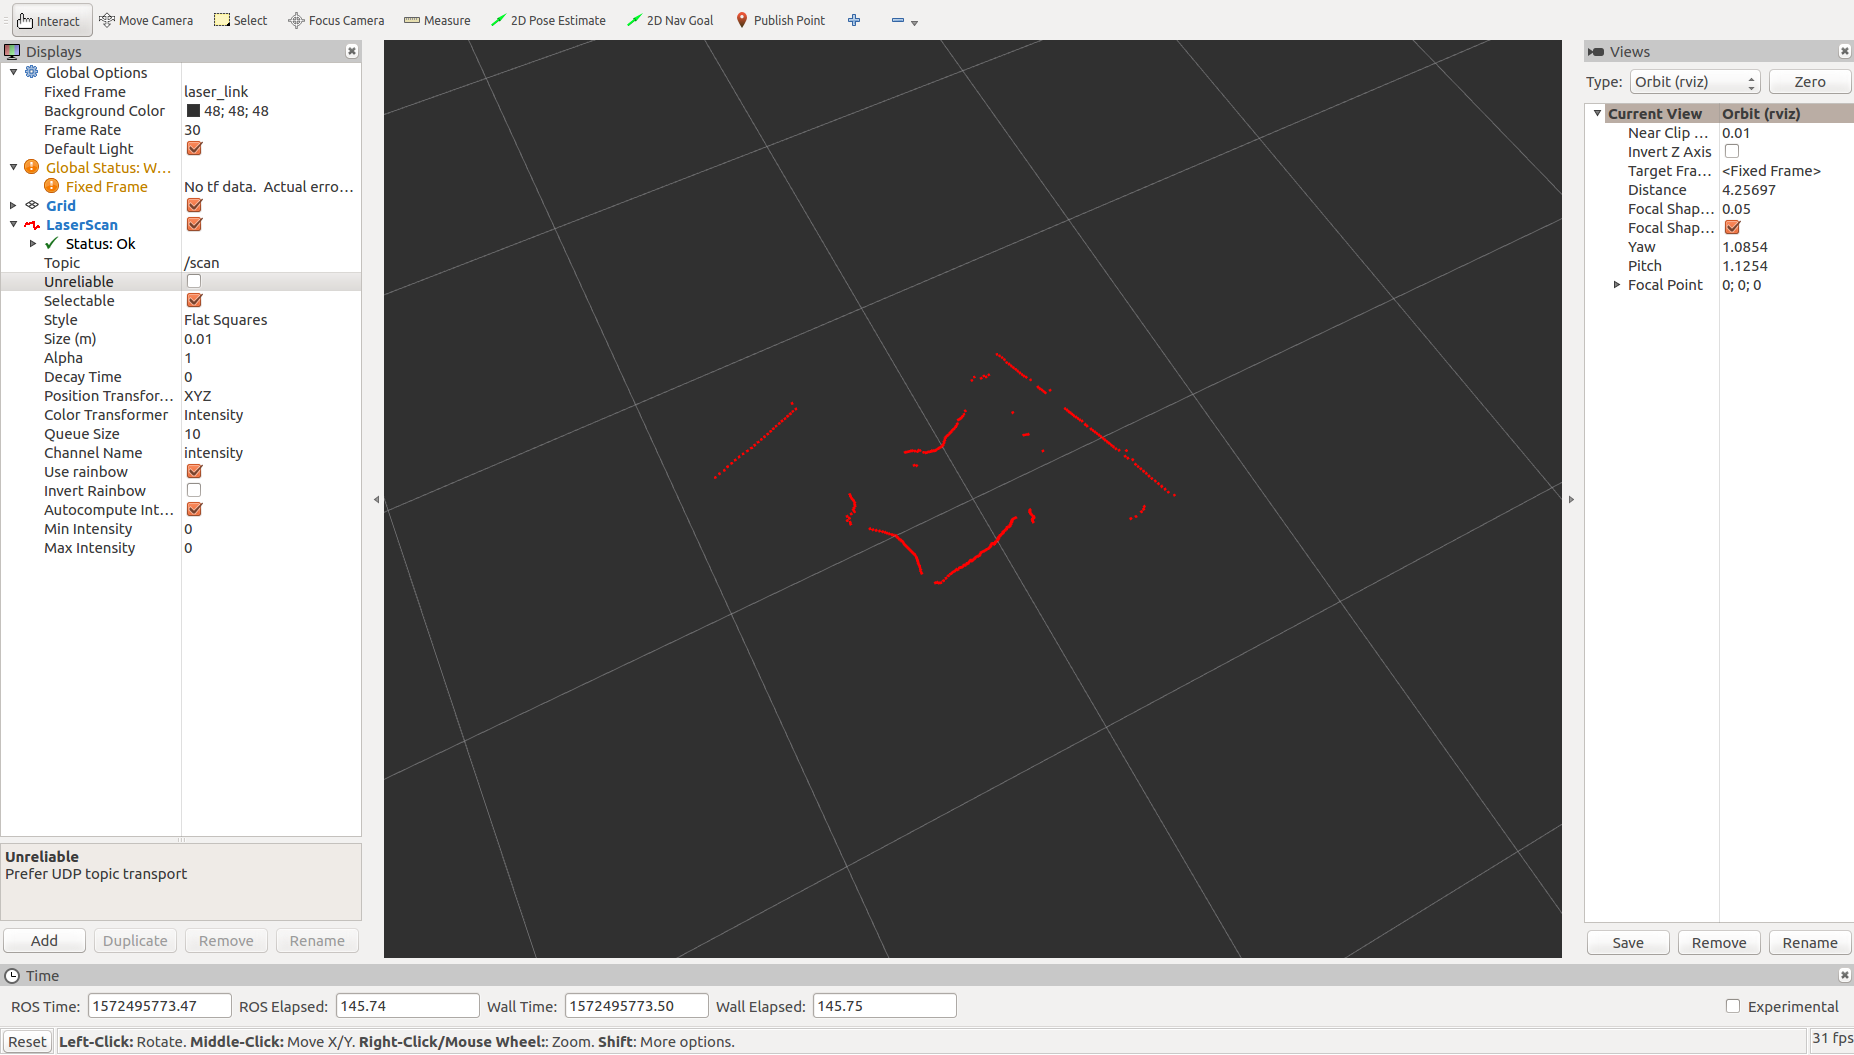
\includegraphics[width=0.5\textwidth]{laser.png}}
\caption{Lidar Data.}
\label{ld}
\end{figure}

The control node of the car is a transplantation of code from existing controller. It's easy to send control commands by publishing commands to corresponding topic. As we can see, it's easy for users to build their projects based on ROS in our platform. Since ROS is widely used, it's important that our platform helps users who want to try ROS.